\documentclass[main.tex]{subfiles}
\begin{document}

\chapter{Contextvrije talen en hun gramatica}
\label{cha:contextvrije-talen}

\section{Contextvrije Grammatica}
\label{sec:contextvrije-grammatica}


\begin{de}
  Een \term{contextvrije grammatica} (\term{CFG}) is een $4$-tal $(V,\Sigma,R,S)$:
  \begin{itemize}
  \item $V$: een eindige verzameling niet-eindsymbolen. (variabelen of non-terminals)
  \item $\Sigma$: een eindig alfabet van eindsymbolen, disjunct met $V$. (terminals)
  \item $R$: een eindige verzameling regels (producties).\\
    Een regel is een koppel van \'e\'en niet-eindsymbool en een string van elementen uit $V \cup \Sigma_{\epsilon}$. We schrijven deze vaak met een $\rightarrow$ ertussen.
  \item $S\in V$: het startsymbool.
  \end{itemize}
\end{de}

\begin{de}
  Zij $c = (V,\Sigma,R,S)$ een CFG.
  Een string $f$ over $V \cup \Sigma_{\epsilon}$ wordt afgeleid uit een string $b$ over $V \cup \Sigma_{\epsilon}$ met behulp van $c$ als er een eindige rij strings $s_{0},\dotsc,s_{n}$ bestaat zodat het volgende geldt:
  \begin{itemize}
  \item $s_{0} = b$
  \item $s_{n} = f$
  \item $s_{i+1}$ wordt verkregen door in $s_{i}$ een niet-eindsymbool $x$ te vervangen door het overeenkomstige eindsymbool in een regel uit $R$.
    We noteren dit proces als volgt.
    \[ \forall i: s_{i} \leadsto s \]
  \end{itemize}
  \[ b \leadsto^{*} f \]
\end{de}

\begin{de}
  De taal $L_{c}$ bepaald door een CFG $c = (V,\Sigma,R,S)$ is de verzameling strings over $\Sigma$ die kunnen afgeleid worden van het startsymbool $S$.
  \[ L_{c} = \{ s \in \Sigma^{*}\ |\ S \leadsto^{*} s \} \]
\end{de}

\begin{de}
  \label{de:contextvrije-taal}
  Een taal $L$ is \term{contextvrij} (een \term{CFL}) als er een CFG bestaat zodat die CFG die taal bepaalt.
  \[ \exists L:\ L = L_{CFG} \]
\end{de}

\begin{de}
  Een \term{meest-linkse} afleiding van een string $s$ uit een CFG $c$ is een afleiding waarbij steeds het meest linkse niet-eindsymbool vervangen is.
\end{de}

\begin{de}
  Zij $c = (V,\Sigma,R,S)$ een CFG en $s$ een string die afgeleid kan worden uit $S$.
  De string $s$ is \term{ambigu} als de meest-linke afleiding van $s$ uit $S$ niet uniek is. 
\end{de}

\begin{de}
  Twee contextvrije grammatica's $c_{1}$ en $c_{2}$ zijn \term{equivalent} als ze dezelfde taal bepalen.
  \[ L_{c_{1}} = L_{c_{2}} \]
\end{de}

\begin{st}
  De equivalentie van contextvrije gramatica's is een equivalentierelatie.

  \begin{proof}
    Inderdaad, de gelijkheid van talen is een equivalentierelatie.
  \end{proof}
\end{st}

\begin{de}
  We noemen een CFG $c = (V,\Sigma,R,S)$ \term{niet ambigu} als er in de taal bepaald door $c$ geen ambigue strings zitten.
\end{de}

\begin{de}
  Een taal noemen we \term{inherent ambigu} als er geen niet-ambigue CFG bestaat die deze taal bepaalt.
\end{de}

\begin{de}
  \label{de:chomsky-normaal-vorm}
  Een CFG $c = (V,\Sigma,R,S)$ heeft de \term{Chomsky Normaal Vorm} als elke regel \'e\'en van de volgende vormen heeft:
  \begin{itemize}
  \item $A \rightarrow BC$ met $A$, $B$ en $C$ niet-eindsymbolen en $B$ en $C$ verschillend van $S$.
  \item $A \rightarrow a$ met $A$ een niet-eindsymbool en $a$ een eindsymbool.
  \item $S \rightarrow \epsilon$
  \end{itemize}
\end{de}

\begin{st}
  \label{st:constructie-chomsky-normaalvorm}
  Voor elke CFG $c = (V,\Sigma,R,S)$ bestaat er een equivalente contextvrije grammatica in Chomsky Normaal Vorm.

  \begin{proof}
    Constructief bewijs.\\
    Kies een willekeurige CFG $c = (V,\Sigma,R,S)$, dan construeren we nu een equivalente CFG $c' = (V',\Sigma,R',S)$ in Chomsky Normaal Vorm.

    \begin{itemize}
    \item Om te beginnen zorgen we ervoor dat in $c'$ het startsymbool enkel links in een regel voorkomt.
      Vervang overal in de regels van $R$ $S$ door een nieuw niet-eindsymbool $X$ en voeg een regel $S\rightarrow X$ toe.
    \item Vervolgens zorgen we dat $\epsilon$ enkel rechtstreeks volgt uit $S$.

      Stel dat we twee regels $\mathcal{Q} = A \rightarrow \epsilon$ en $\mathcal{R} = B \rightarrow \gamma$ kunnen vinden in $R$ waarbij $A$ voorkomt in $\gamma$.
      Definieer een verzameling regels $V(\mathcal{Q},\mathcal{R})$ als de verzameling van de regels van de vorm $B\rightarrow \eta$ waarbij $\eta$ verkregen wordt door in $\gamma$ een combinatie van de voorkomens van $A$ te schrappen.
      Op die manier zijn alle mogelijkheden waarop $\epsilon$ kon voorkomen in de originele regel vervangen door een equivalente regel.

      Pas $c$ nu iteratief aan door elk paar regels $\mathcal{Q}$ en $\mathcal{R}$ te vinden en $V(\mathcal{Q},\mathcal{R})$ toe te voegen aan $R$.
      Deze iteratie is eindig omdat zowel elke opeenvolging van symbolen in een regel eindig is als het aantal regels.
      Verwijder vervolgens alle regels van de vorm $A\rightarrow \epsilon$
      
      De bekomen grammatica bepaalt nog steeds dezelfde taal.
      \clarify{waarom?}

    \item Nu zorgen we ervoor dat er steeds vooruitgang zit in de regels.
      Alle regels van de vorm $A\rightarrow B$ moeten dus weg.

      Stel dat we twee regels $\mathcal{Q} = A \rightarrow B$ en $\mathcal{R} = B \rightarrow \gamma$ kunnen vinden in $R$.
      Defineer een regel $U(\mathcal{Q},\mathcal{R}) = A \rightarrow \gamma$.

      Pas $c$ nu iteratief aan door elk paar regels $\mathcal{Q}$ en $\mathcal{R}$ te vinden en $U(\mathcal{Q},\mathcal{R})$ toe te voegen aan $R$.
      Deze iteratie is eindig omdat het aantal regels in $R$ eindig is.
      Verwijder vervolgens alle regels van de vorm $A\rightarrow B$.

      De bekomen grammatica bepaalt nog steeds dezelfde taal.
      \clarify{waarom?}

    \item Er zijn nu nog vier soorten regels te behandelen:
      \begin{itemize}
      \item $A\rightarrow BC$ met $B$ en $C$ twee niet-eindsymbolen.
        Deze laten we voor wat ze zijn.
      \item $A\rightarrow \gamma$ waarin $\gamma$ bestaat uit minstens twee symbolen.
        Vervang elk eindsymbool $a$ door een nieuw niet-eindsymbool $A_{a}$ en voeg de regel $A_{a} \rightarrow a$ toe.

        Deze procedure is eindig omdat zowel elke opeenvolging van symbolen in een regel eindig is als het aantal regels.

        De bekomen grammatica bepaalt nog steeds dezelfde taal.
        \clarify{waarom?}

      \item $S\rightarrow \epsilon$.
        Deze laten we voor wat ze zijn.
      \item $A\rightarrow c$ met $c$ een eindsymbool.
        Deze laten we ook voor wat ze zijn.
      \end{itemize}
    
    \item Tenslotte maken we nog komaf met de regels van de vorm $A \rightarrow X_{1}\dotsc X_{n}$ met $n > 2$.
      Vervang elke regel van deze vorm door $n$ nieuwe regels:
      \[ A \rightarrow X_{1}Y_{1} \]
      \[ \forall i:\ Y_{i} \rightarrow X_{i+1}Y_{i+1} \]

      Deze procedure is eindig omdat zowel elke opeenvolging van symbolen in een regel eindig is als het aantal regels.

      De bekomen grammatica bepaalt nog steeds dezelfde taal.
      \clarify{waarom?}


    \item Wat er van $R$ overblijft noemen we nu $R'$ en $V'$ is hoogstwaarschijnlijk ook uitgebreid.
    \end{itemize}
  \end{proof}
\end{st}

\begin{st}
  \label{st:chomsky-normaalvorm-afleidingslengte}
  Een afleiding van een string van lengte $n>0$ uit het startsymbool van een contextvrije grammatica in Chomsky normaalvorm heeft lengte $2n-1$.
  \begin{proof}
    Om een string van lengte $n$ af te leiden moet er voor elk symbool $a$ een regel van de vorm $A \rightarrow a$ gevolgd worden.
    Dit zijn dus als $n$ stappen van de afleiding.
    Elk van die $A$ moeten bovendien verkregen zijn door $S$ te `splitsen' in twee.
    Om $S$ te `splitsen' in $n$ stukken door telkens in $2$ te `splitsen' zijn er $n-1$ `splitsingen' nodig.
    De lengte van de afleiding is dus $n + n - 1 = 2n-1$.
  \end{proof}
\end{st}

\begin{de}
  Een CFG $c = (V,\Sigma,R,S)$ heeft de \term{Greibach Normaal Vorm} als elke regel \'e\'en vor de volgende vormen heeft:
  \begin{itemize}
  \item $A \rightarrow aX$ met $A$ een niet-eindsymbool, $X$ een (mogelijk lege) sequentie van niet-eindsymbolen en $a$ een eindsymbool.
  \item $S \rightarrow \epsilon$
  \end{itemize}
\end{de}

\begin{st}
  Voor elke CFG $c = (V,\Sigma,R,S)$ bestaat er een equivalente contextvrije grammatica in Breibach Normaal Vorm.
 
\extra{bewijs}
\end{st}

\begin{st}
  Een afleiding van een string van lengte $n>0$ uit het startsymbool van een contextvrije grammatica in Breibach normaalvorm heeft lengte $n$.
 
  \begin{proof}
    Om een string van lengte $n$ af te leiden moeten er $n$ eindsymbolen te voorschijn komen door het toepassen van de regels van de grammatica.
    In elke stap van de vorm $A \rightarrow aX$ komt er precies \'e\'en eindsymbool te voorschijn.
    Er zijn zo dus $n$ stappen nodig. Bijgevolg is de lengte van de afleiding van een string van lengte $n$ van lengte $n$.
  \end{proof}
\end{st}

\begin{st}
  De taal van contextvrije grammatica's is regulier.

  \begin{proof}
    Definieer eerst $V^{n}$ als $(|_{v \in V}v)^{n}$ voor een verzameling $V$ en $V^{*} = (|_{v \in V}v)^{*}$.
    We construeren nu een reguliere expressie voor de taal van contextvrije grammatica's over $\Sigma$ met niet-eindsymbolen $V$.
    In de constructie moeten we natuurlijk $V$ en $\Sigma$ vervangen door de hele beschrijving ervan, maar die is steeds eindig, dus regulier.\stref{st:eindige-taal-regulier}
    \[
    (V,\Sigma, R, V^{1}) \text{ met } R = \{ (V^{1} \rightarrow (V \cup \Sigma)^{1}) (,(V^{1} \rightarrow V \cup \Sigma)^{1})^{*} \}
    \]
  \end{proof}
\end{st}

\begin{st}
  \label{st:regex-cfl}
  De taal van reguliere expressies is contextvrij maar niet regulier.
  
  \begin{proof}
    De taal van reguliere expressies is niet regulier.
    Een reguliere expressie kan immers oneindig geneste haakjes bevatten.
    De taal is wel contextvrij.
    Hier is namelijk een CFG voor de taal van reguliere expressies over een alfabet $\Sigma$
    \[ (\{E\},\Sigma\cup \{(,),*,|,\epsilon,\phi\},R,E)\]
    Merk op dat de $\epsilon$ hierboven wel degelijk het symbool $\epsilon$ betekent en niet de lege string.
    \[ R =
    \left\{ 
      \begin{array}{l}
        E \rightarrow \epsilon,\\
        E \rightarrow a,\\
        E \rightarrow \phi,\\
        E \rightarrow EE,\\
        E \rightarrow E^{*},\\
        E \rightarrow E|E
      \end{array}
    \right\}
    \]
    \end{proof}
\end{st}

\section{Push-down automaten}
\label{sec:push-down-automaten}

\begin{de}
  Een \term{push-down automaat} (\term{PDA}) is een $6$-tal $(Q,\Sigma,\Gamma,\delta,q_{s},F)$:
  \begin{itemize}
  \item $Q$: een eindige verzameling toestanden.
  \item $\Sigma$: een eindig input alfabet.
  \item $\Gamma$: een eindig stapelalfabet.
  \item $\delta:\ Q\times \Sigma_{\epsilon} \times \Gamma_{\epsilon} \rightarrow \mathcal{P}(Q\times \Gamma_{\epsilon})$: een overgangsfunctie.
  \item $q_{s}$: de starttoestand
  \item $F\subseteq Q$: een verzameling aanvaardbare eindtoestanden.
  \end{itemize}
\end{de}

\begin{de}
  Een string $s$ wordt aanvaardt door een PDA $p = (Q,\Sigma,\Gamma,\delta,q_{s},F)$ als $s$ kan worden opgesplitst in $m$ delen $w_{i}$ zodat er $m+1$ toestanden $q_{j}$ bestaan en $m+1$ stacks $stack_{k}$ zodat het volgende geldt:
  \begin{itemize}
  \item $stack_{0} = \epsilon$: De stack is leeg aan het begin.
  \item $q_{0} = q_{s}$: De automaat start in de begintoestand.
  \item $q_{m} \in F$: De laatste toestand is een aanvaardbare toestand.
  \item $(q_{i+1}, y) \in \delta(q_{i}, w_{i+1}, x)$ waarbij $stack_{i} = xt$ en $stack_{i+1} = yt$ gelden met $t\in \Gamma^{*}$: De overgangen gebeuren volgens $\delta$.
  \end{itemize}
\end{de}

\begin{de}
  De taal $L$ bepaald door een PDA bestaat uit alle strings die door de PDA aanvaard worden.
\end{de}

\begin{lem}
  \label{lem:cfg-naar-pda}
  Vanuit elke CFG kunnen we een PDA construeren die dezelfde taal bepaalt.
\TODO{bewijs}
\end{lem}

\begin{opm}
  Het inputalfabet van een PDA komt overeen met de eindsymbolen van een CFG.
  Het stapelalfabet komt overeen met de unie van de niet-eindsymbolen en de eindsymbolen.
\end{opm}

\begin{lem}
  \label{lem:pda-naar-cfg}
 Vanuit elke PDA kunnen we een CFG construeren die dezelfde taal bepaalt. 
\TODO{bewijs p 71}
\end{lem}

\begin{gev}
  \label{taal-pda-contextvrij}
  Als een taal bepaald wordt door een PDA is die taal contextvrij.
\TODO{bewijs}
\end{gev}

\begin{gev}
  Elke reguliere taal is contextvrij.\\\\
  We kunnen dit op twee manieren bewijzen
  \begin{itemize}
  \item Via een PDA:
    \begin{proof}
      Kies een reguliere taal $L$. Er bestaat dan een NFA $n$ die $L$ bepaalt.\footnote{Zie gevolg \ref{gev:reguliere-taal-NFA}.}
      Beschouw nu de PDA $p$ die $n$ `uitbreidt' door zijn stapel te negeren.
      $p$ bepaalt nu dezelfde taal als $n$, dus $L$ is contextvrij.\footnote{Zie stelling \ref{taal-pda-contextvrij}.}
\clarify{ formeler? }
    \end{proof}
  \item Door rechtstreeks een CFG op te stellen voor een reguliere taal.
    \begin{proof}
      Kies een reguliere taal $L$ over een alfabet $\Sigma$, er bestaat dan een reguliere expressie die $L$ bepaalt.\footnote{Zie eigenschap \ref{ei:reguliere-taal-expressie}.}
      We construeren nu inductief een CFG $c = (V,\Sigma,R,S)$ die ook $L$ bepaalt voor elke mogelijke reguliere expressie.
      $V$ wordt steeds ruim genoeg (maar natuurlijk steeds eindig) gekozen zodat het alle symbolen bevat die in $R$ voorkomen.
      Voor elke vorm van een reguliere expressie construeren we de regels die recursief aan $R$ moeten toegevoegd worden.
      \[
      \begin{array}{|c|c|}
        \hline
        E                           & R\\
        \hline
        a \text{ met } a \in \Sigma & \{ S \rightarrow a \}\\
        \epsilon                    & \{ S \rightarrow \epsilon \} \\
        \phi                        & \emptyset\\
        (E_1E_2)                    & \{ \S \rightarrow S_{1}S_{2} \} \\
        (E)^{*}                      & \{ S \rightarrow \epsilon,\ S \rightarrow S_{1}S \}\\
        (E_1|E_2)                   & \{ S \rightarrow S_{1},\ S \rightarrow S_{2} \}\\
        \hline
      \end{array}
      \]
    \end{proof}
  \end{itemize}
\end{gev}

\begin{st}
  Elke PDA bepaalt een contextvrije taal en elke contextvrije taal wordt bepaald door een PDA.
 
  \begin{proof}
    Inderdaad!\footnote{Zie lemma \ref{lem:cfg-naar-pda}.} \footnote{Zie lemma \ref{lem:pda-naar-cfg}.}
  \end{proof}
\end{st}

\section{Pompend lemma voor contextvrije talen}

\begin{st}
  Voor een contextvrije taal $L$ bestaat een getal $p$ (de pomplengte) zodat elke string $s$ van $L$ met lengte minstens $p$ kan opgedeeld worden in   vijf stukken $u$, $v$, $x$, $y$ en $z$ uit $\Sigma^{*}$
  \[ s = uvxyz \]
  \begin{enumerate}
    \item $\forall i \in \mathbb{N}:\ uv^{i}xy^{i}z \in L$
    \item $|vy| > 0$
    \item $|vxy| < p$
  \end{enumerate}
  \begin{proof}
    Kies een willekeurige contextvrije taal $L$, en bestaat dan een contextvrije grammatica $c'$ die $L$ bepaalt.\footnote{Zie definitie \ref{de:contextvrije-taal}.}
    $c'$ kan nu steeds omgezet worden naar een CFG $c = (V,\Sigma,R,S)$ in Chomsky normaalvorm.\footnote{Zie stelling \ref{st:constructie-chomsky-normaalvorm}.}
    Elke regel heeft nu ofwel precies twee niet-eindsymbolen ofwel geen enkel niet-eindsymbool aan de rechterkant staan.\footnote{Zie definitie \ref{de:chomsky-normaal-vorm}.}
    Noem het aantal niet-eindsymbolen in $c$ $|V| = n$.

    Voor elke string $s$ in $L$ bestaat er nu door $c$ een afleidingsboom. Zie figuur \ref{fig:afleidingsboom}.
    \begin{figure}[H]
      \centering
      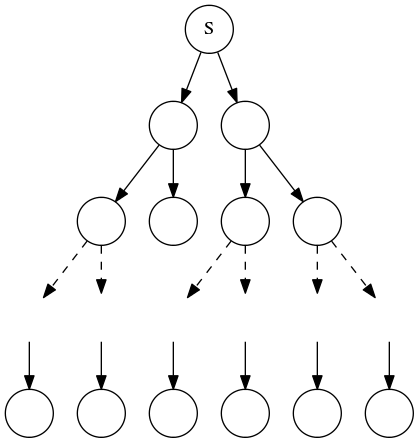
\includegraphics[width=0.5\textwidth]{assets/pompend-lemma-parsetree.png}      
      \caption{De afleidingsboom}
      \label{fig:afleidingsboom}
    \end{figure}
    Omdat de CFG in Chomsky normaalvorm staat kunnen we de onderste takken van de afleidingsboom snoeien om een binaire boom te bekomen. Zie figuur \ref{fig:afleidingsboom-gesnoeid}.
    Deze boom heeft een hoogte van hoogte minstens gelijk aan $\log_{2}(|s|)$.
    Het langste enkelvoudig pad van de wortel van die boom bevat dus $\log_{2}(|s|)+1$ knopen.
    Als $s$ lang genoeg is, is $\log_{2}(|s|) + 1$ groter dan $n$.
    \begin{figure}[H]
      \centering
      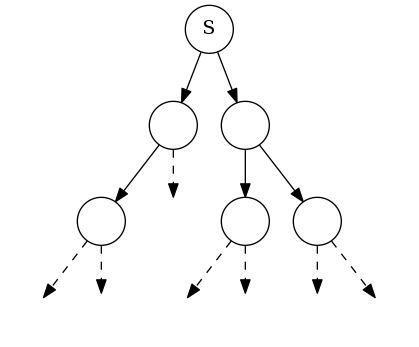
\includegraphics[width=0.5\textwidth]{assets/pompend-lemma-parsetree-gesnoeid.png}      
      \caption{De gesnoeide afleidingsboom}
      \label{fig:afleidingsboom-gesnoeid}
    \end{figure}
    Op dat pad moet er dan minstens \'e\'en niet-eindsymbool, noem het $X$, herhaald worden.
    $X$ is zeker niet $S$, want dan kon $\epsilon$ uit $X$ afgeleid worden, en in de Chomsky normaalvorm kan dat niet.
    Noem de laagste $X$ op dat pad $X_{1}$ en zijn dichtste herhaling $X_{2}$. 
    Zie figuur \ref{fig:afleidingsboom-compact}.
    \begin{figure}[H]
      \centering
      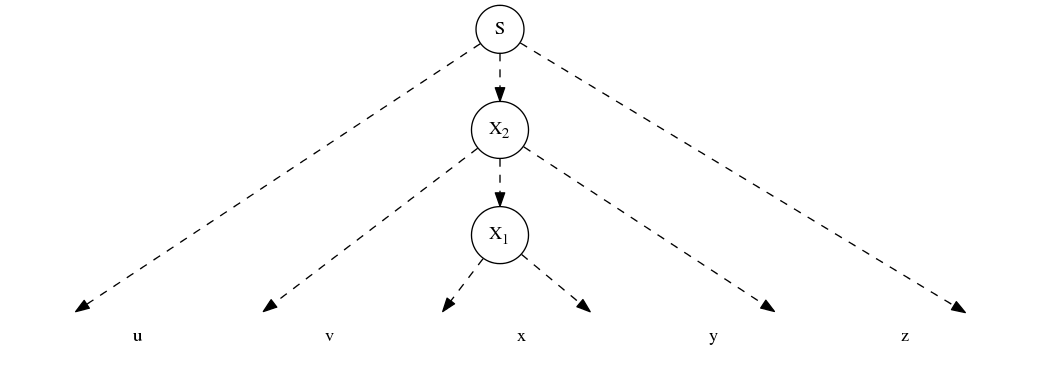
\includegraphics[width=0.8\textwidth]{assets/pompend-lemma-herhaling.png}      
      \caption{De situatie, compact voorgesteld.}
      \label{fig:afleidingsboom-compact}
    \end{figure}
    We kunnen nu de afleiding construeren van $s$ uit $S$ in stukken:
    \[ S \leadsto^{*} uX_{2}z \leadsto^{*} xvX_{1}yz \leadsto^{*} uvxyz \]
    De stukken $u$, $v$, $x$, $y$ en $z$ zijn strings over $\Sigma$.
    $v$ en $y$ kunnen bovendien niet tegelijkertijd leeg zijn, want dan zou $X$ uit zichzelf afgeleidt kunnen worden en dat kan in een Chomsky normaalvorm niet.
    De volgende afleidingen zijn nu ook geldig:
    \[ S \leadsto^{*} uX_{2}z \leadsto^{*} xvX_{1}yz \leadsto^{*} uxz \]
    \[ \forall i \in \mathbb{N}:\ S \leadsto^{*} uX_{2}z \leadsto^{*} xvX_{1}yz \leadsto^{*} xv^{i}X_{1}y^{i}z \]
    Bovenstaande redenering kunnen we opbouwen voor elke string langer dan $2^{(n-1)}$.
    Dit wordt dus de pomplengte $p$.
    \[ p = 2^{(n-1)} \]
    We besluiten nu nog dat $|vxy|$ kleiner is dan $p$.
    De string $vxy$ wordt immers afgeleidt uit $X$ met een afleidingsboom die kleiner is dan $n$ (in hoogte) en bijgevolg hoogstens $2^{n-1}$ bladeren heeft.
    Elk van deze bladeren komt overeen met precies \'e\'en symbool in $vxy$, dus $|vxy| < p$ geldt.
  \end{proof}
\end{st}

\section{Een algebra van contextvrije talen?}

\begin{de}
  De unie $c_{1} \cup c_{2}$ van twee CFG's $c_{1}$ en $c_{2}$ is de CFG die de unie van $L_{c_{1}}$ en $L_{c_{2}}$ bepaalt.
\end{de}

\begin{st}
  \label{st:unie-cfgs-bestaat-altijd}
  De unie $c_{1} \cup c_{2}$ van twee CFG's $c_{1}$ en $c_{2}$ valt steeds eenvoudig te construeren.
  
  \begin{proof}
    Noem $S_{1}$ en $S_{2}$ de startsymbolen van respectievelijk $c_{1}$ en $c_{2}$.
    De unie van $c_{1}$ en $c_{2}$ heeft nu als symbolen de unie van de symbolen van $c_{1}$ en $c_{2}$.
    De unie heeft als regels de unie van de regels van $c_{1}$ en $c_{2}$.
    Merk op dat de symbolen van $c_{2}$ eerst moeten hernoemd worden zodat ze niet overeenkomen met de symbolen van $c_{1}$
    Voeg nu een nieuw symbool $S$ toe alsook de regels $S\rightarrow S_{1}$ en $S\rightarrow S_{2}$ om de unie van $c_{1}$ en $c_{2}$ te vervolledigen.
  \end{proof}
\end{st}

\begin{de}
  De doosnede $c_{1} \cap c_{2}$ van twee CFG's $c_{1}$ en $c_{2}$ is de CFG die de doorsnede van $L_{c_{1}}$ en $L_{c_{2}}$ bepaalt.
\end{de}

\begin{tvb}
  \label{tvb:doorsnede-cfl-niet-altijd-cfl}
  De doorsnede van twee CFG's bestaat niet noodzakelijk.
  De doorsnede van twee contextvrije talen is immers niet steeds contextvrij.\footnote{Het is zelfs niet beslisbaar of de doorsnede van twee contextvrije talen contextvrij is.(zie later)}

  \begin{proof}
    Kies $L_{1} = \{ a^{n}b^{n}c^{m} \ |\ n,m \ge 0 \}$ en $L_{2} = \{ a^{n}b^{m}c^{m} \ |\ n,m \ge 0 \}$.
    De doorsnede $L_{1} \cap L_{2}$ van $L_{1}$ en $L_{2}$ is nu een bekend voorbeeld van een taal die niet contextvrij is.\vbref{vb:0n-1n-2n-niet-contextvrij}
    \[ L_{1} \cap L_{2} = \{ a^{n}b^{n}c^{n} \ |\ n \ge 0 \} \]
  \end{proof}
\end{tvb}

\begin{de}
  Het complement $\bar{c}$ van een CFG $c$ is de CFG die het complement $\bar{L_{c}}$ van $L_{c}$ bepaalt.
\end{de}

\begin{st}
  Het complement van een CFG bestaat niet noodzakelijk.
  Het complement van een contextvrije taal is immers niet steeds contextvrij.\footnote{Het is zelfs niet beslisbaar of het complement van een contextvrije taal contextvrij is.(zie later)}

  \begin{proof}
    De doorsnede $A \cap B$ van twee talen $A$ en $B$ kan geschreven worden als de samenstelling van de unie en het complement.
    Omdat de unie van twee contextvrije talen zeker contextvrij is\stref{st:unie-cfgs-bestaat-altijd}, volgt hieruit dat het complement van twee contextvrije talen niet noodzakelijk contextvrij is.\tvbref{tvb:doorsnede-cfl-niet-altijd-cfl}
  \end{proof}
\end{st}

\begin{gev}
  De verzameling van contextvrije talen vormt geen algebra onder de unie, de doorsnede en het complement.
  Onder enkel de unie vormt de verzameling van contextvrije talen wel een algebra.
\end{gev}

\begin{st}
  De doorsnede van een contextvrije taal en een reguliere taal is een contextvrije taal.
\TODO{bewijs}
\end{st}

\section{Ambigu\"iteit en determinisme}

\begin{de}
  Een contextvrije taal $L$ noemen we \term{deterministisch} als er een deterministische push-down automaat bestaat die $L$ bepaalt.
\end{de}

\begin{de}
  We noteren de verzameling van deterministische contextvrije talen als $DCFL$.
\end{de}

\begin{st}
  Een taal $L$ is deterministisch als $L$ niet inherent ambigu is.
  \begin{proof}
    Inderdaad, een ambigue taal kan onmogelijk deterministisch zijn.
  \end{proof}
\end{st}

\begin{opm}
  Er zijn wel niet-ambigue talen die niet-deterministisch zijn.
\extra{geef een voorbeeld?}
\end{opm}


\section{Contextsensitieve Grammatica}

\begin{de}
  Een \term{contextsensitieve grammatica} (\term{CSG}) is een $4$-tal $(V,\Sigma,R,S)$:
  \begin{itemize}
  \item $V$: een eindige verzameling niet-eindsymbolen. (variabelen of non-terminals)
  \item $\Sigma$: een eindig alfabet van eindsymbolen, disjunct met $V$. (terminals)
  \item $R$: een eindige verzameling regels (producties).\\
    \[ \alpha A \beta \rightarrow \alpha \gamma \beta \text{ met } \alpha, \beta \in (V \cup \Sigma)^{*},\ \gamma \in (V \cup \]
  \item $S\in V$: het startsymbool.
  \end{itemize}
\end{de}


\begin{de}
  Zij $c = (V,\Sigma,R,S)$ een CSG.
  Een string $f$ over $V \cup \Sigma_{\epsilon}$ wordt afgeleid uit een string $b$ over $V \cup \Sigma_{\epsilon}$ met behulp van $c$ als er een eindige rij strings $s_{0},\dotsc,s_{n}$ bestaat zodat het volgende geldt:
  \begin{itemize}
  \item $s_{0} = b$
  \item $s_{n} = f$
  \item $s_{i+1}$ wordt verkregen door in $s_{i}$ een substring $x$ te vervangen door een overeenkomstige substring $y$ van een regel uit $R$.
    We noteren dit proces als volgt.
    \[ \forall i: s_{i} \leadsto s \]
  \end{itemize}
  \[ b \leadsto^{*} f \]
\end{de}

\begin{de}
  De taal $L_{c}$ bepaald door een CSG $c = (V,\Sigma,R,S)$ is de verzameling strings over $\Sigma$ die kunnen afgeleid worden van het startsymbool $S$.
  \[ L_{c} = \{ s \in \Sigma^{*}\ |\ S \leadsto^{*} s \}
\]
\end{de}

\begin{de}
  Een taal $L$ is \term{contextsensitief} (een \term{CSL}) als er een CSG bestaat zodat die CSG die taal bepaalt.
  \[ \exists L:\ L = L_{CSG} \]
\end{de}

\begin{de}
  Een CSG $c = (V,\Sigma,R,S)$ heeft de \term{Kuroda Normaal Vorm} als elke regel \'e\'en van de volgende vormen heeft.
  Zij $A$, $B$, $C$ en $D$ niet-eindsymbolen en $a$ een eindsymbool.
  \begin{itemize}
  \item $AB \rightarrow CD$
  \item $A \rightarrow BC$
  \item $A \rightarrow B$
  \item $A \rightarrow a$
  \end{itemize}
\end{de}

\TODO{ een lineair begrensde automaat LBA }

\TODO{taal van contextsensitieve grammatica's is regulier}


\end{document}